\documentclass[border=3pt]{standalone}
% Preâmbulo compartilhado pelos diagramas TikZ da aula 8 de Navegação (Implementação do RRT)
\usepackage[T1]{fontenc}
\usepackage[utf8]{inputenc}
\usepackage{lmodern}
\usepackage{amsmath}
\usepackage{xcolor}
\usepackage{tikz}
\usetikzlibrary{arrows.meta,angles,quotes,decorations.pathmorphing,decorations.pathreplacing,calc,
                positioning,shapes.geometric,shapes.misc,backgrounds,fit,
                math}

% Paleta (mesma dos SVGs originais)
\definecolor{dblue}{HTML}{2A5B8C}
\definecolor{dorange}{HTML}{B3541E}
\definecolor{dgreen}{HTML}{4A7C59}
\definecolor{dred}{HTML}{9C4B4B}
\definecolor{dcream}{HTML}{F4F1EA}
\definecolor{dshade}{HTML}{DDD7C9}

% Função gaussiana (não normalizada por padrão de escala visual)
\pgfmathdeclarefunction{gauss}{3}{%
  \pgfmathparse{1/(#3*sqrt(2*pi))*exp(-((#1-#2)^2)/(2*#3^2))}%
}

% Estilos comuns (prefixo d... para não colidir com chaves internas do pgf)
\tikzset{
  >={Stealth[length=2mm]},
  dguide/.style={gray!55, dashed, line width=0.4pt},
  daxis/.style={gray!60, line width=0.7pt, ->},
  dbody/.style={fill=black!3, draw=black!80, line width=1pt},
  dacc/.style={draw=dblue, line width=1pt},
  dlbl/.style={black!55, font=\small},
  dsub/.style={black!45, font=\footnotesize},
  dstate/.style={circle, draw=black!80, fill=dcream, line width=1pt,
                 minimum size=17mm, font=\large, inner sep=1pt},
  dobs/.style={circle, draw=black!80, fill=dshade, line width=1pt,
               minimum size=14mm, font=\large, inner sep=1pt},
  dbox/.style={rounded corners=2pt, draw=black!80, fill=dcream, line width=1pt,
               align=center, inner sep=6pt},
  dop/.style={circle, draw=black!80, fill=white, line width=1pt,
              minimum size=6mm, inner sep=0pt, font=\small},
  dtrans/.style={->, dblue, line width=1pt},
  dmeas/.style={->, dorange, line width=1pt},
  dcurve/.style={line width=1pt, dblue},
  dcurveb/.style={line width=1.4pt, dorange},
}

\begin{document}
\hyphenpenalty=10000 \exhyphenpenalty=10000 \tolerance=9999 \emergencystretch=3em
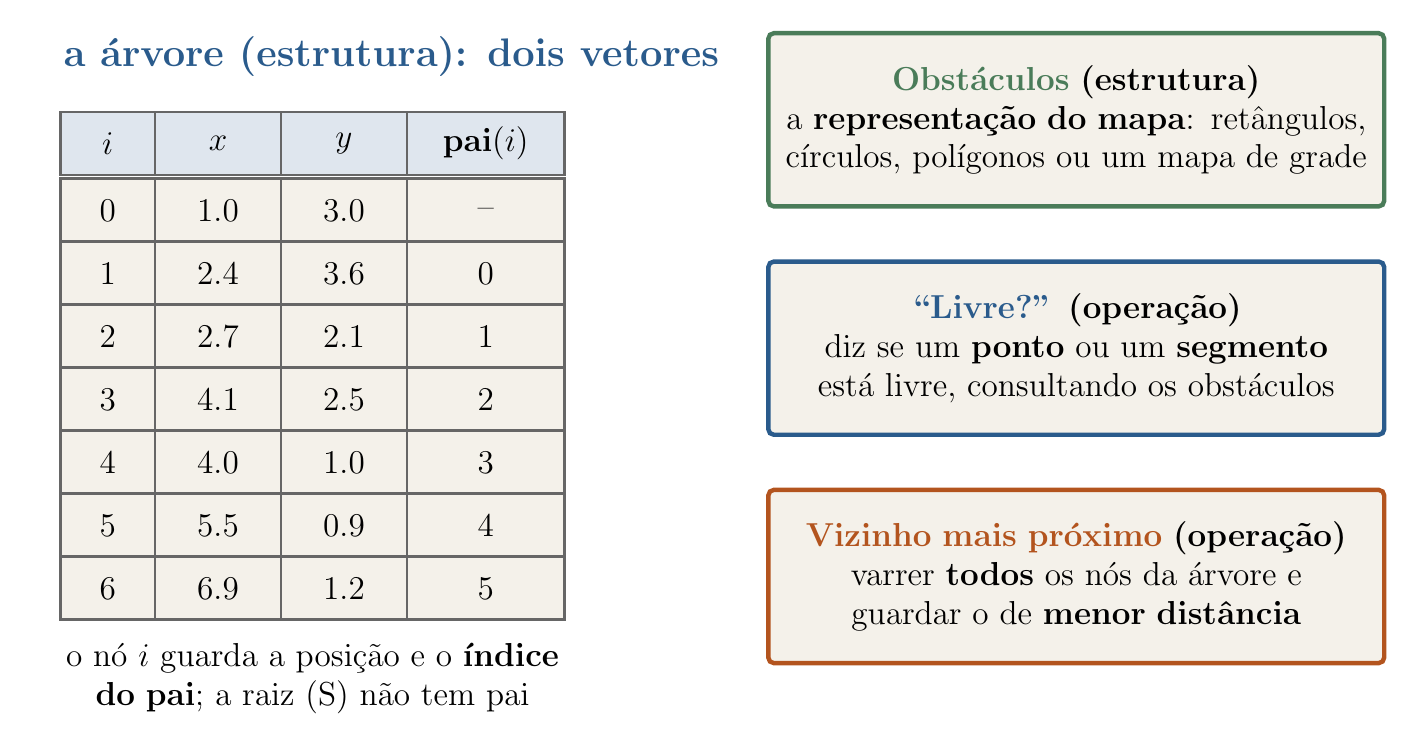
\begin{tikzpicture}[x=1cm,y=1cm]
\node[font=\Large\bfseries, text=dblue] at (4.2,8.2) {a árvore (estrutura): dois vetores};
\tikzset{c/.style={draw=black!60, line width=1pt, minimum height=0.8cm, font=\large, fill=dcream}}
\node[c, minimum width=1.2cm, fill=dblue!15, font=\large\bfseries] at (0.60,7.1) {$i$};
\node[c, minimum width=1.6cm, fill=dblue!15, font=\large\bfseries] at (2.00,7.1) {$x$};
\node[c, minimum width=1.6cm, fill=dblue!15, font=\large\bfseries] at (3.60,7.1) {$y$};
\node[c, minimum width=2.0cm, fill=dblue!15, font=\large\bfseries] at (5.40,7.1) {pai$(i)$};
\node[c, minimum width=1.2cm] at (0.60,6.25) {0};
\node[c, minimum width=1.6cm] at (2.00,6.25) {1.0};
\node[c, minimum width=1.6cm] at (3.60,6.25) {3.0};
\node[c, minimum width=2.0cm] at (5.40,6.25) {--};
\node[c, minimum width=1.2cm] at (0.60,5.45) {1};
\node[c, minimum width=1.6cm] at (2.00,5.45) {2.4};
\node[c, minimum width=1.6cm] at (3.60,5.45) {3.6};
\node[c, minimum width=2.0cm] at (5.40,5.45) {0};
\node[c, minimum width=1.2cm] at (0.60,4.65) {2};
\node[c, minimum width=1.6cm] at (2.00,4.65) {2.7};
\node[c, minimum width=1.6cm] at (3.60,4.65) {2.1};
\node[c, minimum width=2.0cm] at (5.40,4.65) {1};
\node[c, minimum width=1.2cm] at (0.60,3.85) {3};
\node[c, minimum width=1.6cm] at (2.00,3.85) {4.1};
\node[c, minimum width=1.6cm] at (3.60,3.85) {2.5};
\node[c, minimum width=2.0cm] at (5.40,3.85) {2};
\node[c, minimum width=1.2cm] at (0.60,3.05) {4};
\node[c, minimum width=1.6cm] at (2.00,3.05) {4.0};
\node[c, minimum width=1.6cm] at (3.60,3.05) {1.0};
\node[c, minimum width=2.0cm] at (5.40,3.05) {3};
\node[c, minimum width=1.2cm] at (0.60,2.25) {5};
\node[c, minimum width=1.6cm] at (2.00,2.25) {5.5};
\node[c, minimum width=1.6cm] at (3.60,2.25) {0.9};
\node[c, minimum width=2.0cm] at (5.40,2.25) {4};
\node[c, minimum width=1.2cm] at (0.60,1.45) {6};
\node[c, minimum width=1.6cm] at (2.00,1.45) {6.9};
\node[c, minimum width=1.6cm] at (3.60,1.45) {1.2};
\node[c, minimum width=2.0cm] at (5.40,1.45) {5};
\node[font=\large, text width=7cm, align=center] at (3.2,0.3) {o nó $i$ guarda a posição e o \textbf{índice do pai}; a raiz (S) não tem pai};
\node[dbox, draw=dgreen, text width=7.4cm, minimum height=2.2cm, font=\large, line width=1.6pt] at (12.9,7.4) {\textbf{\textcolor{dgreen}{Obstáculos} (estrutura)}\\ a \textbf{representação do mapa}: retângulos, círculos, polígonos ou um mapa de grade};
\node[dbox, draw=dblue, text width=7.4cm, minimum height=2.2cm, font=\large, line width=1.6pt] at (12.9,4.5) {\textbf{\textcolor{dblue}{``Livre?''} (operação)}\\ diz se um \textbf{ponto} ou um \textbf{segmento} está livre, consultando os obstáculos};
\node[dbox, draw=dorange, text width=7.4cm, minimum height=2.2cm, font=\large, line width=1.6pt] at (12.9,1.6) {\textbf{\textcolor{dorange}{Vizinho mais próximo} (operação)}\\ varrer \textbf{todos} os nós da árvore e guardar o de \textbf{menor distância}};
\end{tikzpicture}
\end{document}
